\documentclass[12pt]{article}

%%%%%%%%%%%%%%%%%%%%%%%%%%%%
%%%%%%%%%%%%%%%%%%%%%%%%%%%%
% Load in packages
\usepackage{amsmath}
\usepackage{float}
\usepackage{amssymb}
\usepackage{hyperref}
\usepackage{graphicx}
\usepackage{enumitem}
\usepackage{tikz}
\usepackage{pgfplots}
\pgfplotsset{compat=1.18} % or the latest version you have
\usepgfplotslibrary{fillbetween}
\usepackage[top=1in, bottom=1in, left=1in, right=1in]{geometry}

%%%%%%%%%%%%%%%%%%%%%%%%%%%%
%%%%%%%%%%%%%%%%%%%%%%%%%%%%

\begin{document}

\begin{center}
\Large Chapter 8 Practice Problems

\medskip

\normalsize Elements of Microeconomics (discussion section 4)

\medskip

\small Jamie Hyder
\end{center}

\section*{Question 1}
Consider the market for coffee. The equations for quantity demanded and quantity supplied are as follows:
\begin{align*}
    Q_D &= 100-4P\\
    Q_S &= 5P + 10
\end{align*}
\begin{enumerate}[label=(\alph*)]

    \item Derive the inverse supply and demand equations ($P = ...$)
    \item Graph the inverse supply and demand equations.
    \item Is supply/demand elastic or inelastic in this case?
    \item Solve for the equilibrium price and quantity in this market, and illustrate this equilibrium on your graph.
    \item Indicate where on the graph represents the consumer and producer surplus in this market.
    \item Now, assume that there is a tax levied (on sellers) in the market for coffee in the amount of \$4 per cup. Does the supply or demand curve shift?
    \item What is the new equation for $Q_S$ \textit{and} the inverse supply curve?
    \item Add this new inverse supply curve to your existing graph. 
    \item Has the supply curve shifted left or right? By how much has the curve shifted?
    \item What is the new price faced by buyers in this market with the tax? What is the new price faced by sellers in this market with the tax?
    \item Who bears the largest incidence of the tax, buyers or sellers? Why?
    \item Indicate the areas on the graph which represent the producer surplus, consumer surplus, tax revenue, and dead weight loss.
    \item Calculate the values of the producer surplus, consumer surplus, tax revenue, and dead weight loss after the tax is levied in this market.
    \item Would the dead weight loss increase or decrease if the same tax was levied and (ceteris paribus) $Q_S = \frac{1}{2}P + 10$? What if (ceteris paribus) $Q_D = 100 - P$? Why is this the case? 
\end{enumerate}

\newpage

\textbf{Answer:}

\begin{enumerate}[label = (\alph*)]
    \item \begin{align*}
        Q_D &= 100 - 4P \\\
        4P &= 100 - Q_D \\
        P &= 25 - \frac{1}{4} Q_D
    \end{align*}

    \begin{align*}
        Q_S &= 5P + 10 \\
        5P &= Q_S - 10 \\
        P &= \frac{1}{5}Q_S - 2
    \end{align*}

    \item Graph:
    
    \begin{center}
    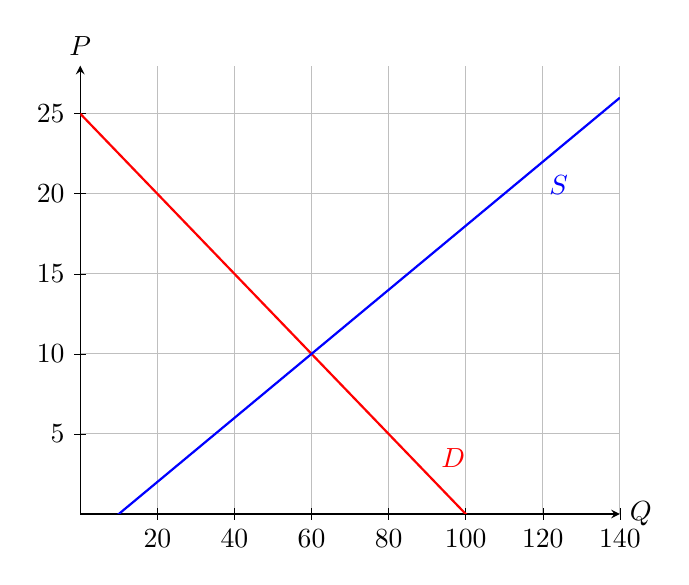
\begin{tikzpicture}
\begin{axis}[
  axis lines=middle,
  xlabel={$Q$},
  ylabel={$P$},
  xmin=0, xmax=140,
  ymin=0, ymax=28,
  domain=0:140,
  samples=200,
  grid=both,
  tick style={black},
  every axis x label/.style={at={(current axis.right of origin)}, anchor=west},
  every axis y label/.style={at={(current axis.above origin)}, anchor=south},
]
  % Demand: P = 25 - 0.25 Q
  \addplot[thick, red] {25 - 0.25*x} node[pos=0.65, above right, red] {$D$};

  % Supply: P = 0.2 Q - 2
  \addplot[thick, blue] {0.2*x - 2} node[pos=0.85, below right, blue] {$S$};

\end{axis}
\end{tikzpicture}
\end{center}

\item Supply is elastic because when price increases by $1$, $Q_S$ increases by $5$ which is more than 1. Demand is also elastic because when price increases by $1$, $Q_D$ decreases by $4$ which is more than 1.

\item 
\begin{align*}
    Q_S &= Q_D \\
    5P + 10 &= 100 - 4P \\
    9P &= 90 \\
    P^* &= 10 \\
    Q_D &= 100 - 4(10) \\
    Q^* & = 60
\end{align*}
$\implies P^* = 10$ and $Q^* = 60$

\vspace{3mm}

\begin{center}
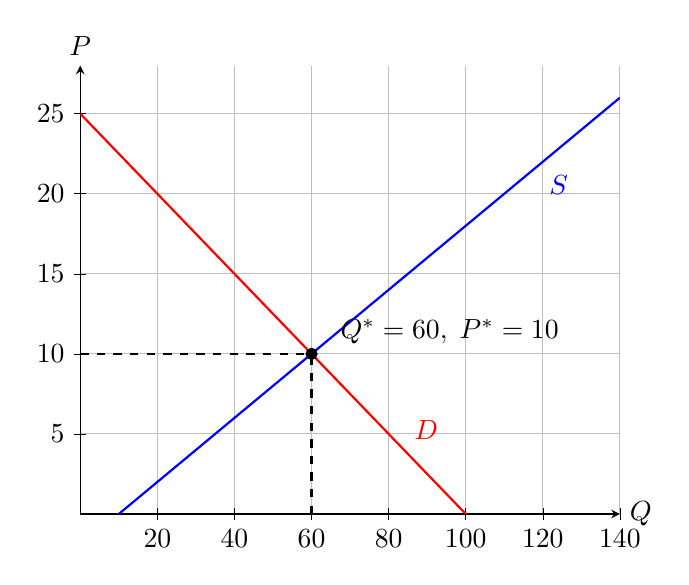
\begin{tikzpicture}
\begin{axis}[
  axis lines=middle,
  xlabel={$Q$},
  ylabel={$P$},
  xmin=0, xmax=140,
  ymin=0, ymax=28,
  domain=0:140,
  samples=200,
  grid=both,
  tick style={black},
  every axis x label/.style={at={(current axis.right of origin)}, anchor=west},
  every axis y label/.style={at={(current axis.above origin)}, anchor=south},
]
  % Demand: P = 25 - 0.25 Q
  \addplot[thick, red] {25 - 0.25*x} node[pos=0.6, above right, red] {$D$};

  % Supply: P = 0.2 Q - 2
  \addplot[thick, blue] {0.2*x - 2} node[pos=0.85, below right, blue] {$S$};

  % Equilibrium point (Q*, P*) = (60, 10)
  \addplot[only marks, mark=*] coordinates {(60,10)};
  \node[anchor=south west] at (axis cs:65,10) {$Q^*=60,\;P^*=10$};

  % Dashed projections to axes
  \addplot[thick, dashed] coordinates {(60,0) (60,10)};
  \addplot[thick, dashed] coordinates {(0,10) (60,10)};
\end{axis}
\end{tikzpicture}
\end{center}

\item Consumer(pink) and producer(blue) surplus in this market in equilibrium:

\begin{center}
    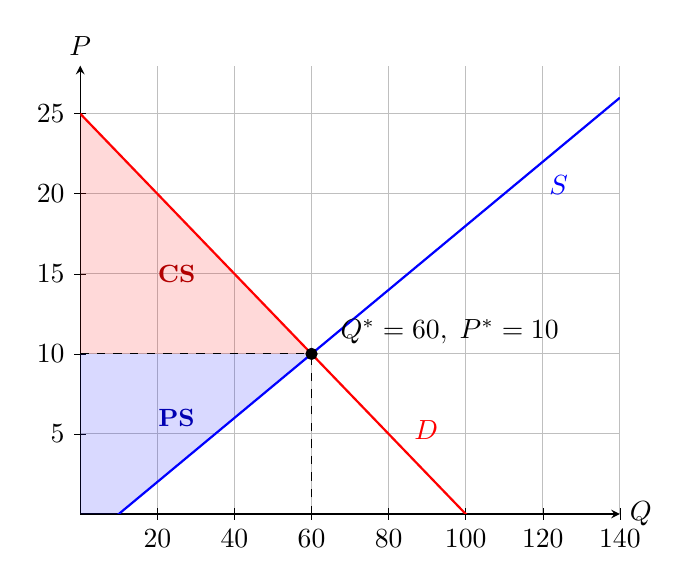
\begin{tikzpicture}
\begin{axis}[
  axis lines=middle,
  xlabel={$Q$},
  ylabel={$P$},
  xmin=0, xmax=140,
  ymin=0, ymax=28,
  domain=0:140,
  samples=200,
  grid=both,
  tick style={black},
  every axis x label/.style={at={(current axis.right of origin)}, anchor=west},
  every axis y label/.style={at={(current axis.above origin)}, anchor=south},
]

  % --- Curves (full range) ---
  % Demand: P = 25 - 0.25 Q
  \addplot[thick, red] {25 - 0.25*x}
    node[pos=0.6, above right, red] {$D$};

  % Supply: P = 0.2 Q - 2
  \addplot[thick, blue] {0.2*x - 2}
    node[pos=0.85, below right, blue] {$S$};

  % --- Define paths restricted to [0, 60] for shading ---
  % Demand segment up to Q*=60
  \addplot[name path=Dseg, draw=none, domain=0:60] {25 - 0.25*x};
  % Supply segment up to Q*=60
  \addplot[name path=Sseg, draw=none, domain=0:60] {0.2*x - 2};
  % Price line at P*=10 up to Q*=60
  \addplot[name path=Pstar, draw=none, domain=0:60] {10};

  % --- Shaded areas ---
  % Consumer Surplus: area between demand and P* from 0 to 60
  \addplot[
    fill=red, fill opacity=0.15, draw=none
  ] fill between[of=Dseg and Pstar];

  % Producer Surplus: area between P* and supply from 0 to 60
  \addplot[
    fill=blue, fill opacity=0.15, draw=none
  ] fill between[of=Pstar and Sseg];

  % --- Equilibrium point and guides ---
  \addplot[only marks, mark=*] coordinates {(60,10)};
  \node[anchor=south west] at (axis cs:65,10) {$Q^*=60,\;P^*=10$};

  \addplot[dashed] coordinates {(60,0) (60,10)};
  \addplot[dashed] coordinates {(0,10) (60,10)};

    % Labels for shaded areas
  \node[red!70!black, font=\small\bfseries] at (axis cs:25,15) {CS};
  \node[blue!70!black, font=\small\bfseries] at (axis cs:25,6) {PS};

\end{axis}
\end{tikzpicture}

\end{center}

\item The supply curve shifts when there is a tax levied.

\item When there is a tax of $\$4 $ per cup, at any given $Q_S$, $P$ will be $\$4 $ higher, so we get \(P = \frac{1}{5}Q_S + 2\) as the new inverse supply curve, and so $Q_S = 5P - 10$.


\item Graph: 

\begin{center}
    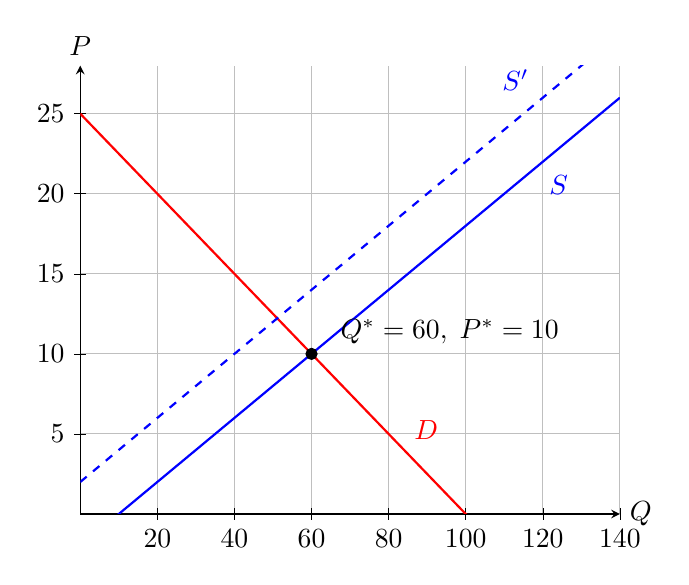
\begin{tikzpicture}
\begin{axis}[
  axis lines=middle,
  xlabel={$Q$},
  ylabel={$P$},
  xmin=0, xmax=140,
  ymin=0, ymax=28,
  domain=0:140,
  samples=200,
  grid=both,
  tick style={black},
  every axis x label/.style={at={(current axis.right of origin)}, anchor=west},
  every axis y label/.style={at={(current axis.above origin)}, anchor=south},
]
  % Demand: P = 25 - 0.25 Q
  \addplot[thick, red] {25 - 0.25*x} node[pos=0.6, above right, red] {$D$};

  % Supply: P = 0.2 Q - 2
  \addplot[thick, blue] {0.2*x - 2} node[pos=0.85, below right, blue] {$S$};

    % New Supply: P = 0.2Q + 2
  \addplot[thick, blue, dashed] {0.2*x + 2}
    node[pos=0.85, above left, blue] {$S'$};

  % Equilibrium point (Q*, P*) = (60, 10)
  \addplot[only marks, mark=*] coordinates {(60,10)};
  \node[anchor=south west] at (axis cs:65,10) {$Q^*=60,\;P^*=10$};
\end{axis}
\end{tikzpicture}
\end{center}

\item The supply curve has shifted left. There has been a shift upward of 4, representing the \$4 increase in price. This comes from the increase in the intercept of the $P$ equation by 4 units. 

\item The new price faced by the buyers is the price at which the new supply curve meets the existing demand curve:
\begin{align*}
    Q_S^{new} &= Q_D \\
    5P - 10 &= 100 - 4P \\
    9P & = 110 \\
    P^{Buyer} & = \frac{110}{9}
\end{align*}

The new $Q_D$ at this price is \(Q_D = 100 - 4(\frac{110}{9}) = \frac{460}{9}\)

So, the price faced by sellers after the tax is the price at which $Q_S = \frac{460}{9}$ *(note that this is the original supply curve):
\begin{align*}
    P &= \frac{1}{5}Q_S - 2 \\
    P & = \frac{1}{5}(\frac{460}{9}) - 2 \\
    P &= \frac{460}{45} - 2 \\
    P^{Seller} &= \frac{370}{45}
\end{align*}

The new price faced by buyers is $P^{Buyer} = \frac{110}{9}$ and the new price faced by sellers is $P^{Seller} = \frac{370}{45}$

\item Buyers pay more of the tax/face the largest incidence of the tax because their demand is less elastic than supply, ie buyers respond less to the change in price than do the sellers.

\item Graph:

\begin{center}
    \begin{tikzpicture}
\begin{axis}[
  axis lines=middle,
  xlabel={$Q$},
  ylabel={$P$},
  xmin=0, xmax=140,
  ymin=0, ymax=28,
  domain=0:140,
  samples=200,
  grid=both,
  tick style={black},
  every axis x label/.style={at={(current axis.right of origin)}, anchor=west},
  every axis y label/.style={at={(current axis.above origin)}, anchor=south},
]

% --- Curves ---
% Demand
\addplot[thick, red] {25 - 0.25*x}
  node[pos=0.86, above right, red] {$D$};
% Original Supply
\addplot[thick, blue] {0.2*x - 2}
  node[pos=0.86, below right, blue] {$S$};
% Tax-inclusive Supply (shifted up by 4)
\addplot[thick, blue, dashed] {0.2*x + 2}
  node[pos=0.86, right, blue] {$S'$};

% --- Key constants ---
% New (post-tax) equilibrium
\def\Qt{51.11}
\def\Pc{12.22}
\def\Pp{8.22}
% Old (pre-tax) equilibrium
\def\Qstar{60}
\def\Pstar{10}

% --- Helper paths for shading (restricted domains) ---
% Up to new Q (Qt) for CS/PS/Tax rectangle
\addplot[name path=D_up, draw=none, domain=0:\Qt] {25 - 0.25*x};
\addplot[name path=S_dn, draw=none, domain=0:\Qt] {0.2*x - 2};
\addplot[name path=Pc_line, draw=none, domain=0:\Qt] {\Pc};
\addplot[name path=Pp_line, draw=none, domain=0:\Qt] {\Pp};

% For DWL region between Qt and Q* bounded by demand and original supply
\addplot[name path=D_tail, draw=none, domain=\Qt:\Qstar] {25 - 0.25*x};
\addplot[name path=S_tail, draw=none, domain=\Qt:\Qstar] {0.2*x - 2};

% --- Shading ---
% Consumer Surplus after tax: area between demand and Pc from 0 to Qt
\addplot[fill=red, fill opacity=0.15, draw=none]
  fill between[of=D_up and Pc_line];

% Producer Surplus after tax: area between Pp and original supply from 0 to Qt
\addplot[fill=blue, fill opacity=0.15, draw=none]
  fill between[of=Pp_line and S_dn];

% Tax Revenue: rectangle between Pc and Pp from 0 to Qt
\addplot[fill=yellow, fill opacity=0.12, draw=none]
  fill between[of=Pc_line and Pp_line];

% Deadweight Loss: between demand and original supply from Qt to Q*
\addplot[fill=green, fill opacity=0.20, draw=none]
  fill between[of=D_tail and S_tail];

% --- Equilibria and guides ---
% Old equilibrium (optional marker)
\addplot[only marks, mark=o] coordinates {(\Qstar,\Pstar)};
\node[anchor=south west] at (axis cs:\Qstar,\Pstar)

% New equilibrium with tax
\addplot[only marks, mark=*] coordinates {(\Qt,\Pc)};
\node[anchor=south west] at (axis cs:\Qt,\Pc)

% Vertical guide at Qt
\addplot[dashed] coordinates {(\Qt,0) (\Qt,\Pc)};
% Horizontal prices Pc and Pp
\addplot[dashed] coordinates {(0,\Pc) (\Qt,\Pc)};
\addplot[dashed] coordinates {(0,\Pp) (\Qt,\Pp)};
% Label the tax wedge
\node[anchor=west] at (axis cs:\Qt+1,(\Pc+\Pp)/2) {$t=4$};

% --- Region labels ---
\node[red!70!black, font=\small\bfseries]   at (axis cs:2,15) {CS};
\node[blue!70!black, font=\small\bfseries]  at (axis cs:5,6)  {PS};
\node[yellow!70, font=\small\bfseries]       at (axis cs:5,10.2){TR};
\node[green!80!black, font=\footnotesize\bfseries]at (axis cs:56,11)  {DWL};

\end{axis}
\end{tikzpicture}
\end{center}

\item Producer surplus:
\begin{align*}
    PS &= 2*\frac{370}{45} + \frac{1}{2}*(\frac{460}{9} - 2)*\frac{370}{45} \\
    PS & = 261.2
\end{align*}

Consumer surplus:
\begin{align*}
    CS & = \frac{1}{2}*(25-\frac{110}{9})*\frac{460}{9} \\
    CS &= 326.5
\end{align*}

Tax Revenue:
\begin{align*}
    TR &= (\frac{110}{9} - \frac{370}{45})*\frac{460}{9} \\
    TR &= 204.4
\end{align*}

Dead weight loss:
\begin{align*}
    DWL &= \frac{1}{2} * (60-\frac{460}{9})*(\frac{110}{9} - \frac{370}{45}) \\
    DWL &= 17.8
\end{align*}

\item If \(Q_S = \frac{1}{2}P + 10\), DWL will decrease because supply has become more inelastic. If $Q_D = 100-P$, DWL will decrease because demand has become more inelastic.

\end{enumerate}

\newpage
\section*{Question 2}
Assume we are in the market for cars, and a tax has been levied on the car manufacturers of size $\$X$. Illustrate the dead weight loss caused by this tax in the following 4 scenarios on a supply/demand graph:
\begin{enumerate}[label = (\alph*)]
    \item Supply is elastic, demand is inelastic
    \item Supply is elastic, demand is elastic
    \item Demand is elastic, supply is inelastic
    \item Demand is elastic, supply is inelastic
\end{enumerate}
\vspace{2mm}
\textbf{Answer:}
See Figure 5 in Chapter 8 of your book for an accurate illustration of what this would look like. 

\section*{Question 3}
Consider the market for twizzlers. Assume demand and supply are both relatively elastic in this market. Illustrate the dead weight loss and tax revenue caused by a tax of the following three sizes:
\begin{enumerate}
    \item \(\$2\) per twizzler
    \item \(\$4\) per twizzler
    \item \(\$6\) per twizzler
\end{enumerate}

What happens to the size of the tax revenue as the size of the tax increases?

\vspace{3mm}

***(Note that I did not give any specific equations for $Q_S$ or $Q_D$, so you can't calculate the DWL or TR, I just want you to show what happens to DWL/TR as the tax per twizzler increases, nothing precise is necessary)

\vspace{4mm}

\textbf{Answer:}
See figure 6 in your book for an illustration of what this would look like. 

As the size of the tax increases, the tax revenue will grow up to a point where it begins to shrink. This is the result of decreasing Quantities being sold in the market as the price gets higher and higher. 
    


\end{document}
